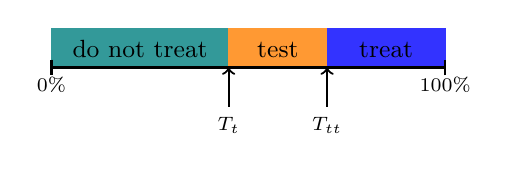
\begin{tikzpicture}
      % \draw[help lines] (-1, -1) grid (6, 1);
      \draw (0,0) node[below] {\scriptsize $0\%$}; 
      \draw (5,0) node[below] {\scriptsize $100\%$};
      \filldraw[teal!80] (0, 0) rectangle +(2.25, 0.5);
      \draw (1.125,0) node[above] {\small do not treat};
      \filldraw[orange!80] (2.25, 0) rectangle +(1.25, 0.5);
      \draw (2.875,0) node[above] {\small test};
      \filldraw[blue!80] (3.5, 0) rectangle +(1.5, 0.5);  
      \draw (4.25,0) node[above] {\small treat};
      \draw[thick] (0, 0) -- (5, 0);
      \draw[thick] (0, 0.1) -- (0, -0.1) ++ (5,0) -- +(0,.2);
      \draw[thick, ->] (2.25, -0.5) node[below] {\scriptsize {$T_t$}} -- +(0, 0.5) ;
      \draw[thick, ->] (3.5, -0.5) node[below] {\scriptsize {$T_{tt}$}} -- +(0, 0.5) ;
\end{tikzpicture}